\documentclass[10pt,twocolumn]{article}
\usepackage[margin=0.75in,columnsep=0.25in]{geometry}
\usepackage[utf8]{inputenc}
\usepackage[T1]{fontenc}
\usepackage{amsmath,amssymb,amsthm}
\usepackage{graphicx}
\usepackage{xcolor}
\usepackage{tikz}
\usetikzlibrary{arrows.meta,positioning,shapes.geometric,fit,backgrounds}
\usepackage{booktabs}
\usepackage{tabularx}
\usepackage{enumitem}
\usepackage{hyperref}

\definecolor{sysblue}{HTML}{1F5AA6}
\definecolor{sysgreen}{HTML}{2C8C62}
\definecolor{sysorange}{HTML}{C97A12}
\definecolor{sysred}{HTML}{B44949}

\newtheorem{definition}{Definition}[section]
\newtheorem{theorem}{Theorem}[section]
\newtheorem{property}{Property}[section]

\newcommand{\sys}{\textsc{Neo-AA}}
\newcommand{\code}[1]{\texttt{\small #1}}
\newcommand{\hash}[1]{\mathcal{H}(#1)}

\setlist[itemize]{leftmargin=*,topsep=2pt,itemsep=1pt}
\setlist[enumerate]{leftmargin=*,topsep=2pt,itemsep=1pt}
\hypersetup{colorlinks=true,linkcolor=blue!60!black,citecolor=blue!60!black,urlcolor=blue!60!black}

\begin{document}

\title{Neo-AA: Cross-Ecosystem Account Abstraction with Heterogeneous Signature Verification}
\author{Anonymous Authors\\\small Submission to IEEE S\&P 2026}
\maketitle

\begin{abstract}
We present \sys, a Neo N3 account-abstraction architecture that unifies native Neo witness authorization with EVM EIP-712 typed signatures inside one shared master contract. The central design challenge is heterogeneity: Neo N3 authorizes transactions through secp256r1-backed witnesses, whereas Ethereum-style workflows authorize through secp256k1 signature recovery over typed data. \sys bridges these models without deploying one wallet contract per user. Instead, it binds each logical account identifier to a deterministic abstract-account address that becomes the user-facing identity, while the logical \code{accountId} remains an internal coordination key for storage, indexing, and verification.

The system contributes four main elements. First, it introduces a mixed authorization protocol that counts Neo witnesses and recovered EVM signer addresses toward one threshold policy. Second, it provides deterministic address generation through a verify-proxy script that routes verification to a shared contract, eliminating per-account deployment costs. Third, it supports human-readable discovery through \code{.matrix} domain resolution and address-based account lookup. Fourth, it exposes a pluggable recovery architecture including Argent-style guardian sets, Safe-style timelocked recovery, Loopring-style guardian-hash recovery, and an oracle-gated dome inactivity flow. We describe the full architecture, state model, workflow, and security properties, and we align the specification with the current implementation and testnet validation pipeline.
\end{abstract}

\section{Introduction}

Account abstraction decouples user identity from cryptographic keys, enabling flexible authorization policies. While Ethereum's ERC-4337 and similar proposals provide single-chain solutions, cross-ecosystem authorization remains unsolved. Neo N3's witness-based transaction model and Ethereum's signature recovery present fundamentally different authorization primitives that cannot be unified through simple bridging.

\subsection{Motivation}

Traditional blockchain accounts tie identity directly to one signing key or to one per-chain smart-wallet deployment. This coupling complicates recovery, fragments user presence across ecosystems, and makes multi-wallet coordination operationally expensive. Neo N3 and EVM ecosystems exacerbate the problem because they expose different authorization primitives, different signing curves, and different transaction assembly workflows.

\subsection{The Neo N3 Challenge}

Neo N3 transactions use a witness array where each witness contains an invocation script and a verification script. Authorization occurs when the verification script (typically checking ECDSA signatures on secp256r1) validates the invocation script against the transaction hash. This model differs fundamentally from Ethereum's approach where signatures are recovered to addresses that are then checked against authorization lists.

A naive cross-chain account abstraction would require:
\begin{itemize}
\item Deploying separate contracts on each chain.
\item Synchronizing authorization state across heterogeneous runtimes.
\item Maintaining chain-specific signing flows with no common threshold semantics.
\end{itemize}

\subsection{Challenges}

\textbf{C1: Heterogeneous Signatures.} Neo N3 uses witness-based authorization with secp256r1, while EVM wallets use EIP-712 typed data and secp256k1 recovery. A unified system must count both schemes without weakening either trust model.

\textbf{C2: Deterministic Addressing.} Per-account deployment is expensive and operationally noisy. A practical design needs stable account addresses without forcing one contract deployment per user.

\textbf{C3: Address-First Usability.} Users typically remember an account address or human-readable domain, not a logical identifier. The account model therefore needs a clean distinction between public account identity and internal storage keys.

\textbf{C4: Recovery and Governance Extensibility.} Production accounts require recoverability, role separation, and policy mutation without hard-coding one recovery scheme into the core contract.

\subsection{Our Solution: Mixed Authorization Protocol}

\sys introduces a \textit{mixed authorization protocol} in which a single Neo N3 master contract accepts both native Neo witnesses and EVM EIP-712 typed signatures and counts them toward one threshold. The key architectural observation is that both signer types can ultimately be normalized into addresses: Neo witnesses are checked with \code{Runtime.CheckWitness}, while EVM signatures are verified on-chain, mapped to recovered Ethereum-style addresses, and evaluated against the same stored role sets.

\textbf{Deterministic Addressing.} Instead of deploying one contract per account, \sys derives a deterministic verify-proxy script that forwards verification to the master contract. Internally, each account is keyed by a logical \code{accountId}; externally, users interact with the deterministic abstract-account address produced from that proxy script. The address is therefore the primary user-facing identity, whereas \code{accountId} remains an internal storage and verification parameter.

\textbf{Address-First Routing.} The implementation exposes both logical-id entrypoints and address-based convenience wrappers, but the common execution path is address-first. Frontends and relayers typically invoke \code{createAccountWithAddress}, \code{executeByAddress}, \code{executeMetaTxByAddress}, \code{getAccountIdByAddress}, and role-discovery getters such as \code{getAccountAddressesByAdmin} and \code{getAccountAddressesByManager}. This organization matches user expectations: users remember the AA account address---or a bound \code{.matrix} domain---rather than an opaque logical identifier.

\textbf{EIP-712 Integration.} EVM signers authorize an operation by signing typed data bound to the AA address, target contract, method hash, argument hash, nonce, and deadline. The contract reconstructs the same digest on-chain, verifies the secp256k1/Keccak256 signatures, derives signer addresses, and feeds the recovered signer set into the same permission engine that serves native Neo execution.

\subsection{Contributions}


This paper makes the following contributions:

\begin{itemize}[leftmargin=*,topsep=2pt,itemsep=1pt]

\item \textbf{Mixed Authorization Protocol}: A unified threshold mechanism that counts both Neo N3 witnesses (secp256r1/SHA256) and EVM EIP-712 signatures (secp256k1/Keccak256) toward a single authorization threshold, enabling cross-ecosystem account abstraction without bridge contracts or state synchronization.

\item \textbf{Deterministic Address Generation}: A zero-deployment account model where verify scripts are deterministically generated and route to a shared master contract, eliminating per-account deployment costs while maintaining address stability.

\item \textbf{Unified Threshold Algorithm}: The CheckMixedSignatures algorithm that seamlessly integrates Neo's Runtime.CheckWitness with EVM signature recovery, supporting pure Neo, pure EVM, and mixed authorization scenarios through a single verification path.

\item \textbf{Formal Security Analysis}: Rigorous security definitions and proofs demonstrating threshold security, replay protection, and authorization correctness under the standard cryptographic assumptions for both signature schemes.

\end{itemize}
\subsection{EVM Integration and Account Management}

\textbf{How EVM Participation Works.} EVM wallets join \sys through EIP-712 typed-data signatures. When an EVM signer authorizes an operation, the signed message commits to the AA account address, target contract, method hash, argument hash, nonce, and deadline. The signature is carried into a Neo transaction, verified on-chain with secp256k1/Keccak256, and converted into a recovered address that can be evaluated against the stored admin or manager sets. If valid, the recovered signer contributes to the same threshold check as any Neo witnesses included in the transaction.

\textbf{Address-First Account Management.} The contract still stores a logical \code{accountId}, but the dominant external interface is address-based. The common creation path is \code{createAccountWithAddress(accountId, accountAddress, ...)}, which creates the logical record and binds it immediately to its deterministic proxy address. The contract also exposes \code{createAccountBatch} for batched logical account creation, as well as bidirectional lookup methods such as \code{getAccountIdByAddress} and \code{getAccountAddress}. This split keeps internal storage compact while preserving an address-oriented user experience.

\textbf{Role Discovery and Indexing.} Rather than forcing users to remember account identifiers, the master contract maintains address-centric discovery indexes. The current implementation exposes role-specific queries such as \code{getAccountsByAdmin}, \code{getAccountsByManager}, \code{getAccountAddressesByAdmin}, and \code{getAccountAddressesByManager}. The first pair returns logical identifiers for internal coordination; the second pair returns the bound AA addresses that users actually recognize and transact with.

\textbf{Transaction Structure Reference.} For detailed transaction layouts showing Pure Neo, Pure EVM, and mixed Neo+EVM flows, see \code{docs/TRANSACTION\_LAYOUTS.md}. Those layouts complement the present specification by showing the concrete Neo script, signer, and witness composition that realizes the abstract protocol described here.

\subsection{.matrix Domain Integration}

\sys integrates with the Matrix naming system as a discovery layer, not as an authorization root. When a user enters \code{alice.matrix}, the frontend resolves the domain owner from the Matrix contract, queries the AA contract for bound addresses associated with that owner, and presents the discovered AA accounts for selection. A typical resolution flow is:

\begin{enumerate}
\item Resolve the \code{.matrix} domain to its owner address through the Matrix contract.
\item Query \code{getAccountAddressesByAdmin(ownerAddress)} and \code{getAccountAddressesByManager(ownerAddress)} on the AA contract.
\item Merge, de-duplicate, and present the resulting bound AA addresses.
\item Load the selected AA account and continue all subsequent execution through the account address.
\end{enumerate}

This separation is intentional: domains improve usability and discovery, while the authoritative authorization state remains on-chain in the AA contract's role and policy storage.

\subsection{Recovery Verifier Architecture}

Neo-AA supports pluggable recovery verifiers through a standardized interface. Each account can optionally set a recovery verifier contract that implements:

\begin{verbatim}
interface IRecoveryVerifier {
  bool verifyRecovery(
    byte[] accountId,
    byte[] operation,
    byte[] proof
  );
}
\end{verbatim}

We implement three recovery models:

\textbf{Argent-Style Guardian Recovery.} Guardians are stored as a set of addresses with a threshold. Recovery requires $m$-of-$n$ guardian signatures on a recovery operation. The verifier stores:
\begin{itemize}[leftmargin=*,topsep=2pt,itemsep=1pt]
\item Guardian address set (serialized)
\item Guardian threshold (uint)
\item Pending recovery operations with timelock
\end{itemize}


\textbf{Argent-Style Guardian Recovery - Detailed Design.}

The Argent recovery model implements a social recovery mechanism where trusted guardians can collectively authorize account recovery operations. The verifier maintains the following on-chain state:

\begin{itemize}[leftmargin=*,topsep=2pt,itemsep=1pt]
\item \textbf{Guardian Set}: Serialized array of guardian addresses, stored as \code{byte[]} to support both Neo and EVM addresses
\item \textbf{Guardian Threshold}: Minimum number of guardian signatures required ($m$ out of $n$ guardians)
\item \textbf{Pending Operations}: Map of recovery operation hashes to pending recovery requests
\item \textbf{Timelock Period}: Configurable delay (default: 24 hours) between initiation and execution
\end{itemize}

\textbf{Recovery Operation Lifecycle:}

\textit{Phase 1: Initiation.} A guardian initiates recovery by calling \code{initiateRecovery(accountId, newAdmins, newThreshold)}. The verifier:
\begin{enumerate}[leftmargin=*,topsep=2pt,itemsep=1pt]
\item Verifies the caller is in the guardian set
\item Computes operation hash: $h = H(\text{accountId} \| \text{newAdmins} \| \text{newThreshold} \| \text{nonce})$
\item Stores pending operation with timestamp and initiator signature
\item Emits \code{RecoveryInitiated} event
\end{enumerate}

\textit{Phase 2: Guardian Approval.} Additional guardians approve by calling \code{approveRecovery(operationHash, signature)}. The verifier:
\begin{enumerate}[leftmargin=*,topsep=2pt,itemsep=1pt]
\item Verifies signature against operation hash
\item Verifies signer is in guardian set and has not already approved
\item Increments approval count for the operation
\item Emits \code{RecoveryApproved} event
\end{enumerate}

\textit{Phase 3: Execution.} Once threshold is met and timelock expires, anyone can call \code{executeRecovery(operationHash)}. The verifier:
\begin{enumerate}[leftmargin=*,topsep=2pt,itemsep=1pt]
\item Verifies approval count $\geq$ threshold
\item Verifies timelock period has elapsed: $\text{Runtime.Time} - \text{initiationTime} \geq T_{\text{lock}}$
\item Returns true to master contract, which updates account admins and threshold
\item Deletes pending operation and increments nonce
\end{enumerate}

\textit{Cancellation.} The current account owner can cancel pending recovery at any time by performing any authorized transaction, which resets all pending operations.



\textbf{Safe-Style Threshold Timelock - Detailed Design.}

The Safe recovery model extends Argent with enhanced timelock flexibility and modular execution. Key design elements:

\begin{itemize}[leftmargin=*,topsep=2pt,itemsep=1pt]
\item \textbf{Configurable Timelock}: Each account can set custom timelock periods (minimum: 1 hour, maximum: 30 days)
\item \textbf{Execution Window}: After timelock expires, recovery must execute within a validity window (default: 7 days)
\item \textbf{Multi-Step Recovery}: Supports partial admin replacement, allowing gradual transition rather than complete takeover
\end{itemize}

The Safe verifier adds execution window validation: after timelock $T_{\text{lock}}$ expires, the operation remains valid for window period $T_{\text{window}}$. Execution fails if $\text{Runtime.Time} > \text{initiationTime} + T_{\text{lock}} + T_{\text{window}}$.

\textbf{Loopring-Style Guardian Hash - Detailed Design.}

The Loopring model prioritizes guardian privacy by storing only a commitment hash on-chain. The verifier maintains:

\begin{itemize}[leftmargin=*,topsep=2pt,itemsep=1pt]
\item \textbf{Guardian Hash}: $H_g = H(\text{guardian}_1 \| \text{guardian}_2 \| \ldots \| \text{guardian}_n \| \text{threshold})$
\item \textbf{Recovery Nonce}: Prevents replay of revealed guardian sets across multiple recovery attempts
\end{itemize}

\textbf{Recovery with Hash Revelation:}

\textit{Phase 1: Initiation with Revelation.} The initiator calls \code{initiateRecovery(accountId, guardianSet, threshold, signatures)}. The verifier:
\begin{enumerate}[leftmargin=*,topsep=2pt,itemsep=1pt]
\item Computes $H_{\text{revealed}} = H(\text{guardianSet} \| \text{threshold})$
\item Verifies $H_{\text{revealed}} = H_g$ (stored hash)
\item Verifies each signature in \code{signatures} against the recovery operation hash
\item Verifies signature count $\geq$ threshold
\item Stores pending operation with revealed guardian set
\end{enumerate}

\textit{Phase 2: Execution.} After timelock, \code{executeRecovery} verifies the revealed guardian set matches the stored hash and executes the recovery operation.

This design prevents guardian enumeration attacks while maintaining verifiable recovery authorization.



\subsection{Dome Inactivity Recovery Protocol}

The dome mechanism provides last-resort recovery for accounts with prolonged inactivity. The protocol involves:

\textbf{Inactivity Detection.} The system tracks the last activity timestamp for each account:
$$\text{lastActivity}[\text{accountId}] = \text{Runtime.Time}$$

An account is considered inactive if:
$$\text{Runtime.Time} - \text{lastActivity}[\text{accountId}] > T_{\text{inactivity}}$$

where $T_{\text{inactivity}}$ is configurable per account (default: 180 days).

\textbf{Oracle-Gated Initiation.} A designated recovery address can initiate dome recovery, but execution requires oracle approval:

\begin{verbatim}
function initiateDomeRecovery(accountId) {
  require(msg.sender == domeRecoveryAddr[accountId])
  require(isInactive(accountId))

  requestId = hash(accountId, Runtime.Time)
  pendingRecovery[requestId] = {
    accountId: accountId,
    initiator: msg.sender,
    timestamp: Runtime.Time,
    status: "pending_oracle"
  }

  emit DomeRecoveryInitiated(requestId, accountId)
}
\end{verbatim}

\textbf{Oracle Validation.} An authorized oracle verifies inactivity and signs approval. After oracle approval, a timelock period (default: 7 days) must elapse. During this period, the original owner can cancel by performing any transaction.



\textbf{1. Heterogeneous Signature Verification.} Mixed authorization protocol unifying Neo N3 witnesses and EVM EIP-712 signatures.

\textbf{2. Deterministic Addressing.} Zero per-account deployment cost via shared master contract.

\textbf{3. Security Analysis.} Formal proofs under discrete logarithm assumption.

\textbf{4. Practical Deployment.} Validated implementation on Neo N3 testnet.



\section{Account Model and Lifecycle}

\subsection{Account Creation and Structure}

An abstract account in \sys is a shared-contract wallet instance with two identifiers: a logical \code{accountId} and a deterministic AA address. The \code{accountId} is the internal storage key and verification parameter; the deterministic AA address is the public, user-facing identity. This separation is central to the implementation and to the user experience: users fund, discover, and invoke the AA through its address, while the contract keeps the logical identifier for compact indexing, address derivation, and compatibility with internal verification routines.

\textbf{Identity Model.}
\begin{itemize}
\item \textbf{Logical identity:} \code{accountId} is created once, validated, and used as the canonical key for durable storage.
\item \textbf{Operational identity:} the deterministic AA address is the signer identity that wallets, relayers, and downstream contracts interact with.
\item \textbf{Binding layer:} the master contract maintains both \code{accountId} $\rightarrow$ \code{accountAddress} and \code{accountAddress} $\rightarrow$ \code{accountId} mappings.
\item \textbf{User-facing rule:} after creation, account operations should prefer the AA address; \code{accountId} is primarily retained for creation, storage, and verifier compatibility.
\end{itemize}

\textbf{Account Creation Flow.}

\begin{enumerate}
\item The client chooses an \code{accountId} and deterministically derives the corresponding AA verify-proxy address.
\item The common creation path invokes \code{createAccountWithAddress(accountId, accountAddress, admins, adminThreshold, managers, managerThreshold)}.
\item The master contract validates that the logical identifier is fresh, the supplied address matches the deterministic proxy derivation, and the role thresholds are well formed.
\item The contract stores the admin and manager sets under the canonical storage key for \code{accountId}, initializes activity tracking, and binds the bidirectional address mappings.
\item The transaction sender is automatically inserted into the admin set when not already present, ensuring that bootstrap creation cannot strand the account.
\end{enumerate}

The contract also supports \code{createAccountBatch} for batched logical-account initialization under shared role parameters. In that mode, the contract still validates role thresholds and still defaults the sender into the admin set when no explicit administrators are supplied. Batch creation is therefore an efficiency tool, not a separate trust model.

% Figure 1: System Architecture Overview
\begin{figure*}[t]
\centering
\small
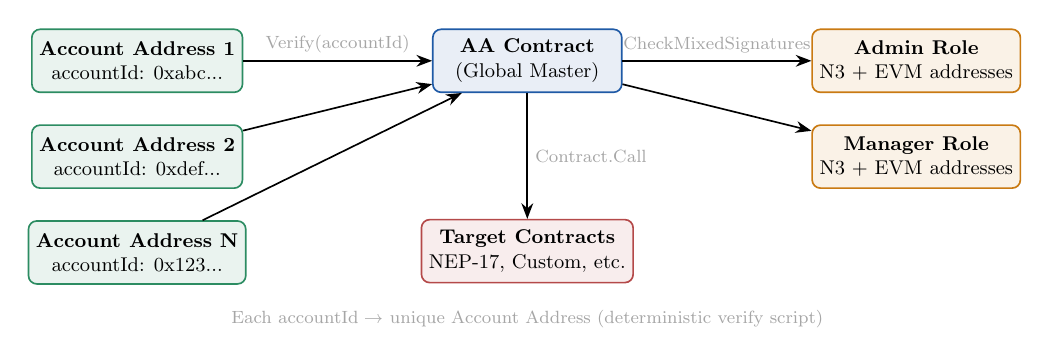
\begin{tikzpicture}[scale=0.8,transform shape,
  node distance=0.8cm and 1.2cm,
  component/.style={draw,rectangle,rounded corners=3pt,minimum width=3cm,minimum height=1cm,font=\small,align=center,line width=0.6pt},
  contract/.style={component,fill=sysblue!10,draw=sysblue},
  account/.style={component,fill=sysgreen!10,draw=sysgreen},
  role/.style={component,fill=sysorange!10,draw=sysorange},
  target/.style={component,fill=sysred!10,draw=sysred},
  arr/.style={-{Stealth[length=2mm,width=1.5mm]},line width=0.6pt},
  label/.style={font=\footnotesize,text=gray!70}
]

% AA Contract (center)
\node[contract] (aa) at (0,0) {\textbf{AA Contract}\\(Global Master)};

% Account Addresses (left)
\node[account,left=3cm of aa] (acc1) {\textbf{Account Address 1}\\accountId: 0xabc...};
\node[account,below=0.5cm of acc1] (acc2) {\textbf{Account Address 2}\\accountId: 0xdef...};
\node[account,below=0.5cm of acc2] (acc3) {\textbf{Account Address N}\\accountId: 0x123...};

% Roles (right)
\node[role,right=3cm of aa] (admin) {\textbf{Admin Role}\\N3 + EVM addresses};
\node[role,below=0.5cm of admin] (manager) {\textbf{Manager Role}\\N3 + EVM addresses};

% Target Contracts (bottom)
\node[target,below=2cm of aa] (target) {\textbf{Target Contracts}\\NEP-17, Custom, etc.};

% Arrows
\draw[arr] (acc1) -- node[above,label] {Verify(accountId)} (aa);
\draw[arr] (acc2) -- (aa);
\draw[arr] (acc3) -- (aa);

\draw[arr] (aa) -- node[above,label] {CheckMixedSignatures} (admin);
\draw[arr] (aa) -- (manager);

\draw[arr] (aa) -- node[right,label] {Contract.Call} (target);

% Legend
\node[label,below=0.3cm of target] {Each accountId → unique Account Address (deterministic verify script)};

\end{tikzpicture}
\caption{Neo-AA system architecture. A shared master contract governs many deterministic AA addresses while storing role sets and authorization policies in one on-chain control plane.}
\label{fig:architecture}
\end{figure*}


\subsection{Deterministic Address Generation}

Each abstract account has a deterministic Neo address derived from its \code{accountId} and the master contract hash. That deterministic address is the account's public identity, signer handle, and discovery key.

\textbf{Verify-Proxy Construction.}

The exact bytecode is produced by the contract's \code{BuildVerifyProxyScript(accountId)} helper. At a logical level, the proxy script performs the following steps:

{\small
\begin{verbatim}
push accountId
push "verify"
push masterContractHash
syscall System.Contract.Call
\end{verbatim}
}

Conceptually, the proxy script:
\begin{enumerate}
\item Carries the logical \code{accountId} into the verification call.
\item Routes verification to the shared AA master contract rather than to a per-account contract instance.
\item Causes the script hash of the proxy to become the externally visible AA address.
\item Allows downstream contracts to rely on \code{Runtime.CheckWitness(accountAddress)} once an authorized AA execution path has opened the proper verification context.
\end{enumerate}

\textbf{Address Derivation.}

The Neo address is computed as:
$$\text{address} = \text{Base58Check}(\text{version} \| \text{Hash160}(\text{verifyScript}))$$

where \code{version = 0x35} for Neo N3 addresses. In implementation terms, the script hash is derived from the proxy bytecode and then reversed into Neo's \code{UInt160} representation before Base58Check encoding for display.

\textbf{Key Properties.}

\begin{itemize}
\item \textbf{Deterministic:} the same \code{accountId} always yields the same verify-proxy address.
\item \textbf{Zero deployment cost:} no per-account contract deployment transaction is required.
\item \textbf{Address-first usability:} the account can be funded, discovered, and referenced by address immediately after derivation.
\item \textbf{Binding integrity:} the contract refuses to bind an \code{accountId} to any address other than the deterministic proxy address derived from that identifier.
\end{itemize}

\subsection{Transaction Structure and Verification Entry}

\textbf{All transactions using an abstract account MUST include the deterministic verify address as a signer.} This triggers the verification entry point in the master contract.

\textbf{Standard Neo-Only Transaction Structure:}

\begin{enumerate}[leftmargin=*,topsep=2pt,itemsep=1pt]
\item \textbf{Script}: Invokes the canonical address-based runtime entry \code{executeUnifiedByAddress(accountAddress, targetContract, method, args, ...)}
\item \textbf{Signers}: Array containing the deterministic verify address (script hash)
\item \textbf{Witnesses}: Array of witness objects, each containing:
  \begin{itemize}[leftmargin=*,topsep=2pt,itemsep=1pt]
  \item \textbf{Invocation Script}: Typically empty or contains signature data
  \item \textbf{Verification Script}: The deterministic verify script (pushes accountId and calls master contract)
  \end{itemize}
\end{enumerate}

\textbf{Verification Entry Flow:}

When Neo consensus nodes process the transaction:
\begin{enumerate}[leftmargin=*,topsep=2pt,itemsep=1pt]
\item Node executes verification script for each witness
\item Verification script calls \code{masterContract.verify(accountId)}
\item Master contract's \code{verify} method:
  \begin{itemize}[leftmargin=*,topsep=2pt,itemsep=1pt]
  \item Checks if calling context is a self-invocation (transaction script calls back to master contract)
  \item Validates transaction script targets an approved wrapper method
  \item Returns \code{true} if valid, \code{false} otherwise
  \end{itemize}
\item If verification succeeds, transaction proceeds to application phase
\item Application phase executes the transaction script, which calls the wrapper method
\item Wrapper method performs authorization check (admin/manager threshold) and policy enforcement
\item If authorized, wrapper invokes the target contract
\end{enumerate}

This two-phase design (verification + application) ensures that:
\begin{itemize}[leftmargin=*,topsep=2pt,itemsep=1pt]
\item Deterministic verify address cannot be misused for unauthorized external calls
\item All operations go through the master contract's policy enforcement layer
\item Authorization state remains centralized and auditable
\end{itemize}
% Figure: Two-Phase Verification Model
\begin{figure}[htbp]
\centering
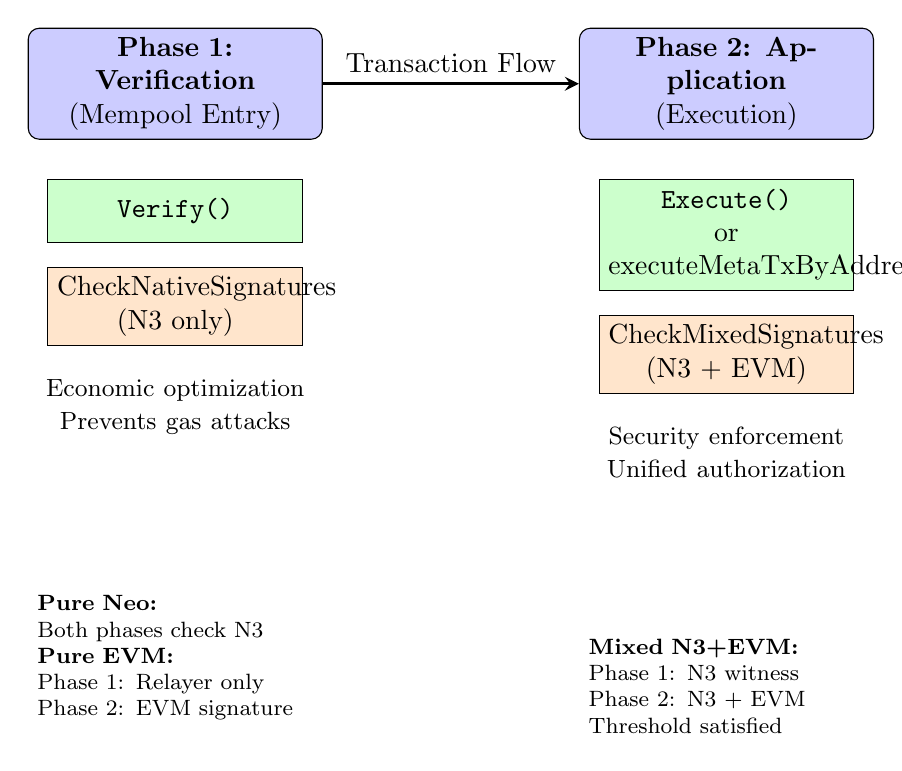
\begin{tikzpicture}[
    node distance=1.5cm,
    phase/.style={rectangle, draw, fill=blue!20, text width=3.5cm, align=center, minimum height=1.2cm, rounded corners},
    method/.style={rectangle, draw, fill=green!20, text width=3cm, align=center, minimum height=0.8cm},
    check/.style={rectangle, draw, fill=orange!20, text width=3cm, align=center, minimum height=0.8cm},
    arrow/.style={->, >=stealth, thick}
]

% Phase 1: Verification
\node[phase] (phase1) at (0,0) {\textbf{Phase 1: Verification}\\(Mempool Entry)};
\node[method, below=0.5cm of phase1] (verify) {\texttt{Verify()}};
\node[check, below=0.3cm of verify] (checkn3) {CheckNativeSignatures\\(N3 only)};
\node[text width=3.5cm, align=center, below=0.3cm of checkn3] (purpose1) {\small Economic optimization\\Prevents gas attacks};

% Phase 2: Application
\node[phase] (phase2) at (7,0) {\textbf{Phase 2: Application}\\(Execution)};
\node[method, below=0.5cm of phase2] (execute) {\texttt{Execute()}\\or\\executeMetaTxByAddress()};
\node[check, below=0.3cm of execute] (checkmixed) {CheckMixedSignatures\\(N3 + EVM)};
\node[text width=3.5cm, align=center, below=0.3cm of checkmixed] (purpose2) {\small Security enforcement\\Unified authorization};

% Timeline arrow
\draw[arrow, very thick] (phase1.east) -- (phase2.west) node[midway, above] {Transaction Flow};

% Annotations
\node[text width=3.5cm, align=left, below=1.8cm of purpose1, font=\footnotesize] (note1) {
\textbf{Pure Neo:}\\
Both phases check N3\\
\textbf{Pure EVM:}\\
Phase 1: Relayer only\\
Phase 2: EVM signature
};

\node[text width=3.5cm, align=left, below=1.8cm of purpose2, font=\footnotesize] (note2) {
\textbf{Mixed N3+EVM:}\\
Phase 1: N3 witness\\
Phase 2: N3 + EVM\\
Threshold satisfied
};

\end{tikzpicture}
\caption{Two-phase verification in Neo-AA. The verification trigger authenticates native Neo paths, while the application trigger combines Neo and EVM signers for mixed authorization.}
\label{fig:two_phase_verification}
\end{figure}


\subsection{Mixed Authorization Transaction Anatomy}

Mixed authorization transactions combine Neo witnesses with EVM EIP-712 signatures. The transaction structure extends the standard Neo transaction with embedded EVM signature data.

\textbf{Mixed Transaction Structure:}

\begin{enumerate}[leftmargin=*,topsep=2pt,itemsep=1pt]
\item \textbf{Script}: Invokes the canonical unified runtime entry \code{executeUnifiedByAddress(accountAddress, targetContract, method, args, signerKeys, argsHash, nonce, deadline, signatures)}
\item \textbf{Signers}: Deterministic verify address (same as Neo-only transactions)
\item \textbf{Attributes}: Custom transaction attribute containing:
  \begin{itemize}[leftmargin=*,topsep=2pt,itemsep=1pt]
  \item EVM signature (65 bytes: $r$, $s$, $v$)
  \item Nonce (per-EVM-signer counter)
  \item Deadline (Unix timestamp)
  \end{itemize}
\item \textbf{Witnesses}: Neo witnesses (may be empty if only EVM authorization is used)
\end{enumerate}

\textbf{EVM Signature Verification in Mixed Transactions:}

The master contract's \code{executeMetaTxByAddress} method:
\begin{enumerate}[leftmargin=*,topsep=2pt,itemsep=1pt]
\item Reconstructs EIP-712 typed data hash from parameters
\item Recovers EVM public key from signature: $\text{pubkey} = \text{ecrecover}(\text{typedDataHash}, r, s, v)$
\item Derives Ethereum address: $\text{addr}_{\text{EVM}} = \text{Keccak256}(\text{pubkey})[12:32]$
\item Validates nonce: retrieves $n_{\text{stored}}$ from storage, verifies $n_{\text{provided}} = n_{\text{stored}}$
\item Validates deadline: verifies $\text{Runtime.Time} \leq \text{deadline}$
\item Checks if $\text{addr}_{\text{EVM}}$ is in admin or manager set
\item Counts valid EVM signature toward threshold
\item Counts valid Neo witnesses toward threshold
\item Accepts if total valid signatures $\geq$ threshold
\end{enumerate}

\subsection{Detailed Verification Flow}

The mixed authorization mechanism is implemented in the \code{CheckMixedSignatures} method, which unifies EVM and Neo signature validation into a single threshold check.

\textbf{Algorithm: CheckMixedSignatures(roles, threshold, verifiedSigners)}

\begin{enumerate}[leftmargin=*,topsep=2pt,itemsep=1pt]
\item Initialize counter: $\text{count} \gets 0$
\item For each role address $r$ in roles:
  \begin{enumerate}[leftmargin=*,topsep=2pt,itemsep=1pt]
  \item \textbf{Check EVM signatures}: If $r \in \text{verifiedSigners}$, then $\text{count} \gets \text{count} + 1$, continue to next role
  \item \textbf{Check Neo witnesses}: If \code{Runtime.CheckWitness(r)} returns true, then $\text{count} \gets \text{count} + 1$
  \end{enumerate}
\item Return $\text{count} \geq \text{threshold}$
\end{enumerate}

\textbf{Key Properties:}

\begin{itemize}[leftmargin=*,topsep=2pt,itemsep=1pt]
\item \textbf{Unified Counting}: EVM signatures and Neo witnesses contribute equally to the threshold
\item \textbf{Priority Order}: EVM signatures are checked first; if matched, Neo witness check is skipped for that role
\item \textbf{Flexible Composition}: Supports pure N3 (all witnesses), pure EVM (all signatures), or mixed scenarios
\end{itemize}

\textbf{Example Scenarios:}

\textit{Scenario 1: Pure N3 Account}
\begin{itemize}[leftmargin=*,topsep=2pt,itemsep=1pt]
\item Configuration: $\text{admins} = [\text{addr}_{\text{N3}}]$, $\text{threshold} = 1$
\item Transaction: Neo witness for $\text{addr}_{\text{N3}}$
\item Verification: \code{CheckWitness(addr\_N3)} returns true, count = 1 $\geq$ 1, authorized
\end{itemize}

\textit{Scenario 2: Pure EVM Account}
\begin{itemize}[leftmargin=*,topsep=2pt,itemsep=1pt]
\item Configuration: $\text{admins} = [\text{addr}_{\text{EVM}}]$, $\text{threshold} = 1$
\item Transaction: EIP-712 signature from $\text{addr}_{\text{EVM}}$
\item Verification: $\text{addr}_{\text{EVM}} \in \text{verifiedSigners}$, count = 1 $\geq$ 1, authorized
\end{itemize}

\textit{Scenario 3: Mixed Account (threshold=2)}
\begin{itemize}[leftmargin=*,topsep=2pt,itemsep=1pt]
\item Configuration: $\text{admins} = [\text{addr}_{\text{N3}}, \text{addr}_{\text{EVM}}]$, $\text{threshold} = 2$
\item Transaction: Neo witness for $\text{addr}_{\text{N3}}$ + EIP-712 signature from $\text{addr}_{\text{EVM}}$
\item Verification: 
  \begin{enumerate}[leftmargin=*,topsep=2pt,itemsep=1pt]
  \item Check $\text{addr}_{\text{N3}}$: not in verifiedSigners, but \code{CheckWitness} returns true, count = 1
  \item Check $\text{addr}_{\text{EVM}}$: in verifiedSigners, count = 2
  \item Result: count = 2 $\geq$ 2, authorized
  \end{enumerate}
\end{itemize}

\textbf{Key Differences from Neo-Only Transactions:}

\begin{itemize}[leftmargin=*,topsep=2pt,itemsep=1pt]
\item EVM signatures are embedded in transaction attributes, not in witnesses
\item EVM signature verification happens during application phase, not verification phase
\item Nonce management is explicit for EVM signers, implicit for Neo witnesses
\item Both signature types count toward the same unified threshold
\end{itemize}

\section{Mixed Authorization Protocol}

\subsection{Protocol Overview}

The mixed authorization protocol operates in four phases:

\textbf{Phase 1: EVM Signature Generation (Off-chain).} The EVM signer constructs EIP-712 typed data and signs with their Ethereum wallet. The signature is a 65-byte value $(r, s, v)$ where $r, s \in \mathbb{F}_p$ are ECDSA signature components and $v \in \{27, 28\}$ is the recovery identifier.

\textbf{Phase 2: Transaction Construction.} A Neo transaction is built with:
\begin{itemize}[leftmargin=*,topsep=2pt,itemsep=1pt]
\item Script: \code{CALLT} to master contract wrapper method
\item Signers: Deterministic verify address for the account
\item Attributes: EVM signature embedded as custom transaction attribute
\item Witnesses: Placeholder for Neo signers
\end{itemize}

\textbf{Phase 3: Neo Witness Collection.} Neo signers add witnesses to the transaction. Each witness contains an invocation script (typically empty or containing the signature) and a verification script (the deterministic proxy script).

\textbf{Phase 4: On-Chain Verification.} The master contract:
\begin{enumerate}[leftmargin=*,topsep=2pt,itemsep=1pt]
\item Validates the deterministic proxy witness
\item Counts Neo witnesses in the authorization set
\item Recovers EVM public key from signature and typed data hash
\item Derives Ethereum address from recovered public key
\item Checks if derived address is in authorization set
\item Accepts if total valid signatures $\geq$ threshold
\end{enumerate}



\subsection{Core Verification Methods}

The Abstract Account contract implements three fundamental verification methods that form the foundation of the mixed authorization protocol. These methods handle different verification scenarios and execution phases.

\subsubsection{Verify Method: Two-Phase Verification Model}

The \code{Verify(accountId)} method is the unified verification entrypoint called by the deterministic proxy script. It implements a two-phase verification model that distinguishes between transaction validation and application execution.

\textbf{Method Signature:}
\begin{small}
\begin{verbatim}
public static bool Verify(ByteString accountId)
Location: AbstractAccount.AccountLifecycle.cs:66-113
\end{verbatim}
\end{small}

\textbf{Two-Phase Verification Architecture:}

The Neo VM verification system operates in two distinct phases (triggers), each with different capabilities and constraints:

\textbf{Phase 1: Verification Trigger (Transaction Validation Phase)}

\begin{itemize}[leftmargin=*,topsep=2pt,itemsep=1pt]
\item \textbf{Timing}: Occurs when a transaction enters the memory pool, before execution
\item \textbf{Purpose}: Validate transaction legitimacy and signature authorization
\item \textbf{Verification Method}: Only \code{Runtime.CheckWitness()} can be used to check Neo native signatures
\item \textbf{EVM Signature Limitation}: Cannot verify EVM signatures in this phase because EIP-712 signature data is in transaction parameters, and the Verification phase cannot access Application data
\item \textbf{Verify Method Behavior}: Checks if transaction shape matches the standard AA wrapper call, then verifies if Neo signatures satisfy the threshold using \code{CheckNativeSignatures}
\end{itemize}

\textbf{Phase 2: Application Trigger (Application Execution Phase)}

\begin{itemize}[leftmargin=*,topsep=2pt,itemsep=1pt]
\item \textbf{Timing}: Occurs during transaction execution when target contract calls \code{Runtime.CheckWitness(accountAddress)}
\item \textbf{Purpose}: Verify if the current execution path has authority to represent the abstract account
\item \textbf{Verification Method}: Checks \code{VerifyContext} to ensure only the target contract pre-authorized by Execute/ExecuteMetaTx can pass
\item \textbf{Verify Method Behavior}: Returns true if and only if the caller is the target contract pre-authorized by the current active execution path
\end{itemize}

\textbf{Different Verification Paths for Neo and EVM Signatures:}

\begin{itemize}[leftmargin=*,topsep=2pt,itemsep=1pt]
\item \textbf{Neo Signatures}: Verified in Verification phase via \code{Runtime.CheckWitness()}
\item \textbf{EVM Signatures}: Verified in Application phase via EIP-712 verification in \code{ExecuteMetaTx}, then counted by \code{CheckMixedSignatures}
\item \textbf{Mixed Authorization}: \code{CheckMixedSignatures} counts both EVM signatures (verifiedSigners) and Neo signatures (CheckWitness) to implement unified threshold checking
\end{itemize}


\subsubsection{CheckNativeSignatures: Pure Neo Signature Verification}

The \code{CheckNativeSignatures} method handles pure Neo native signature verification using only \code{Runtime.CheckWitness()}. This method is used in the Verification phase and for pure Neo execution paths.

\textbf{Method Signature:}
\begin{small}
\begin{verbatim}
private static bool CheckNativeSignatures(
    List<UInt160> roles, 
    int threshold
)
Location: AbstractAccount.ExecutionAndPermissions.cs:252-261
\end{verbatim}
\end{small}

\textbf{Usage Scenarios:}

\begin{itemize}[leftmargin=*,topsep=2pt,itemsep=1pt]
\item Called by \code{Verify} method during Verification phase (transaction validation)
\item Called by \code{Execute/ExecuteByAddress} during Application phase (pure Neo execution path)
\item Any authorization check that only requires Neo native signatures
\end{itemize}

\textbf{Algorithm:}

\begin{small}
\begin{verbatim}
CheckNativeSignatures(roles, threshold):
  Input:  roles     - List of authorized Neo addresses
          threshold - Minimum required signatures
  Output: Boolean indicating whether threshold is satisfied
  
  if threshold <= 0 or roles is null or empty:
    return false
  
  count ← 0
  for each address in roles:
    if Runtime.CheckWitness(address):
      count <- count + 1
  
  return count >= threshold
\end{verbatim}
\end{small}

\textbf{Runtime.CheckWitness Mechanism:}

\begin{itemize}[leftmargin=*,topsep=2pt,itemsep=1pt]
\item Checks if the transaction's \code{Signers} field contains the specified address
\item Verifies the corresponding signature in the \code{Witnesses} field is cryptographically valid
\item Can only be used in Verification and Application phases
\item Cannot verify EIP-712 signatures (EVM signatures are in transaction parameters, not in Witnesses)
\end{itemize}

\textbf{Difference from CheckMixedSignatures:}

\begin{itemize}[leftmargin=*,topsep=2pt,itemsep=1pt]
\item \textbf{CheckNativeSignatures}: Only checks Neo signatures, cannot handle EVM signatures
\item \textbf{CheckMixedSignatures}: Checks both Neo and EVM signatures for mixed authorization
\end{itemize}

\subsection{CheckMixedSignatures: Unified Threshold Algorithm}

The core innovation of the mixed authorization protocol is the \code{CheckMixedSignatures} algorithm, which unifies Neo witness verification and EVM signature verification into a single threshold check. This algorithm is implemented in \code{AbstractAccount.ExecutionAndPermissions.cs:281-315}.

\textbf{Algorithm Definition:}

\begin{small}
\begin{verbatim}
CheckMixedSignatures(roles, threshold, verifiedSigners):
  Input:  roles          - List of authorized addresses (UInt160[])
          threshold      - Minimum required signatures (int)
          verifiedSigners - EVM addresses recovered from signatures (UInt160[])
  Output: Boolean indicating whether threshold is satisfied
  
  count ← 0
  for each address in roles:
    matched ← false
    
    // Step 1: Check if address is an EVM signer
    if verifiedSigners != null:
      for each signer in verifiedSigners:
        if address == signer:
          count <- count + 1
          matched ← true
          break
    
    // Step 2: If not EVM, check for Neo witness
    if not matched:
      if Runtime.CheckWitness(address):
        count <- count + 1
  
  return count >= threshold
\end{verbatim}
\end{small}

\textbf{Key Properties:}

\begin{itemize}[leftmargin=*,topsep=2pt,itemsep=1pt]
\item \textbf{Signature Isolation}: EVM signatures are verified independently using secp256k1/Keccak256, Neo witnesses use secp256r1/SHA256. The two verification paths never interfere.
\item \textbf{Unified Counting}: Regardless of signature origin, each valid signature increments the same counter.
\item \textbf{Threshold Enforcement}: The algorithm returns true if and only if the total count meets or exceeds the configured threshold.
\item \textbf{Order Independence}: The algorithm iterates through the roles list, not the signature list, ensuring consistent behavior regardless of signature submission order.
\end{itemize}
% Figure: CheckMixedSignatures Algorithm
\begin{figure}[htbp]
\centering
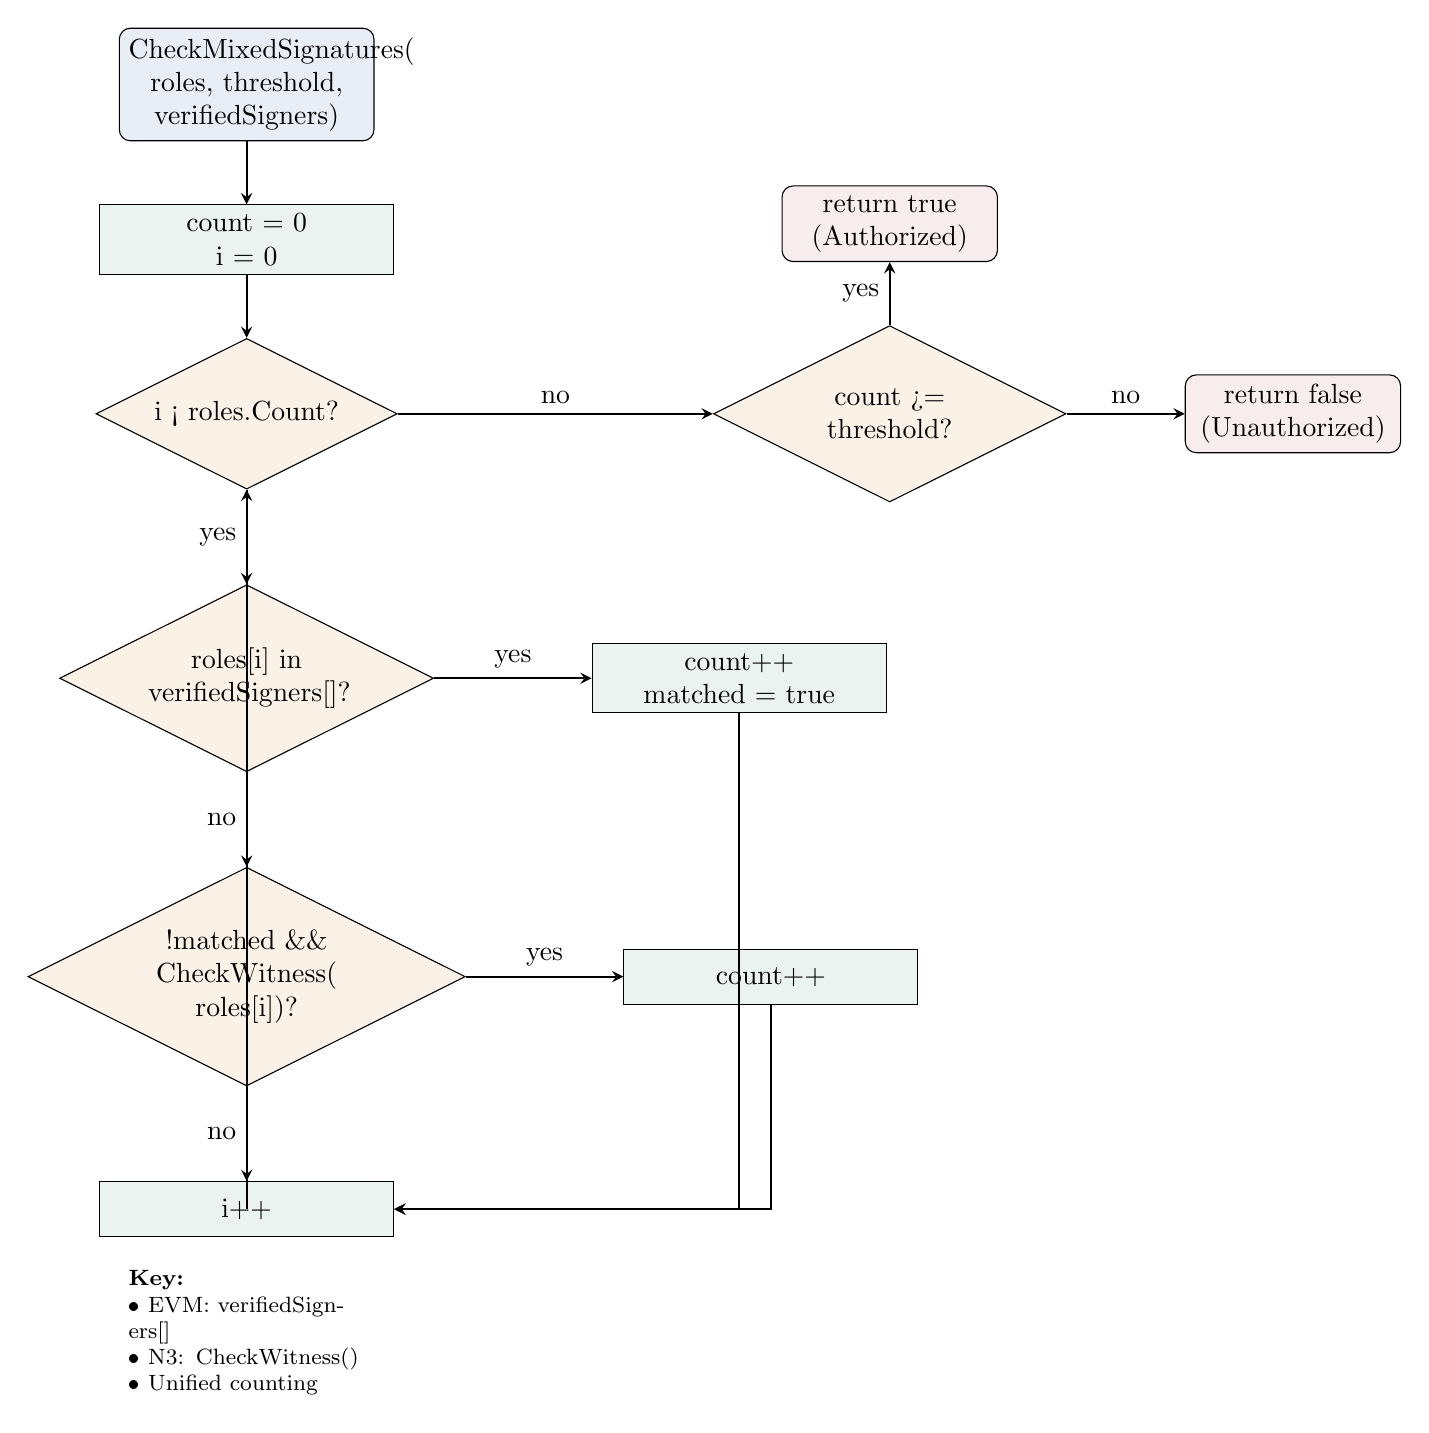
\begin{tikzpicture}[
    node distance=0.8cm,
    start/.style={rectangle, rounded corners, draw, fill=sysblue!10, text width=3cm, align=center, minimum height=0.8cm},
    process/.style={rectangle, draw, fill=sysgreen!10, text width=3.5cm, align=center, minimum height=0.7cm},
    decision/.style={diamond, draw, fill=sysorange!10, text width=2.5cm, align=center, aspect=2},
    result/.style={rectangle, rounded corners, draw, fill=sysred!10, text width=2.5cm, align=center, minimum height=0.7cm},
    arrow/.style={->, >=stealth, thick}
]

% Start
\node[start] (start) at (0,0) {CheckMixedSignatures(\\roles, threshold, verifiedSigners)};

% Initialize
\node[process, below=of start] (init) {count = 0\\i = 0};

% Loop condition
\node[decision, below=of init] (loop) {i < roles.Count?};

% Check EVM signature
\node[decision, below=1.2cm of loop] (checkevm) {roles[i] in\\verifiedSigners[]?};

% Count EVM
\node[process, right=2cm of checkevm] (countevm) {count++\\matched = true};

% Check N3 signature
\node[decision, below=1.2cm of checkevm] (checkn3) {!matched \&\&\\CheckWitness(\\roles[i])?};

% Count N3
\node[process, right=2cm of checkn3] (countn3) {count++};

% Increment
\node[process, below=1.2cm of checkn3] (increment) {i++};

% Final check
\node[decision, right=4cm of loop] (final) {count >=\\threshold?};

% Results
\node[result, above=0.8cm of final] (true) {return true\\(Authorized)};
\node[result, right=1.5cm of final] (false) {return false\\(Unauthorized)};

% Arrows
\draw[arrow] (start) -- (init);
\draw[arrow] (init) -- (loop);
\draw[arrow] (loop) -- node[left] {yes} (checkevm);
\draw[arrow] (loop) -- node[above] {no} (final);
\draw[arrow] (checkevm) -- node[above] {yes} (countevm);
\draw[arrow] (checkevm) -- node[left] {no} (checkn3);
\draw[arrow] (countevm) |- (increment);
\draw[arrow] (checkn3) -- node[above] {yes} (countn3);
\draw[arrow] (checkn3) -- node[left] {no} (increment);
\draw[arrow] (countn3) |- (increment);
\draw[arrow] (increment) -| (loop);
\draw[arrow] (final) -- node[left] {yes} (true);
\draw[arrow] (final) -- node[above] {no} (false);

% Annotations
\node[text width=3cm, align=left, font=\footnotesize, below=0.3cm of increment] (note) {
\textbf{Key:}\\
• EVM: verifiedSigners[]\\
• N3: CheckWitness()\\
• Unified counting
};

\end{tikzpicture}
\caption{Unified threshold evaluation in CheckMixedSignatures. Recovered EVM signers and Neo witnesses are counted against one policy threshold.}
\label{fig:checkmixed_algorithm}
\end{figure}


\subsection{Three Authorization Scenarios}

The mixed authorization protocol supports three distinct operational modes, each demonstrating different aspects of the unified threshold mechanism.
% Figure: Transaction Type Comparison
\begin{figure}[htbp]
\centering
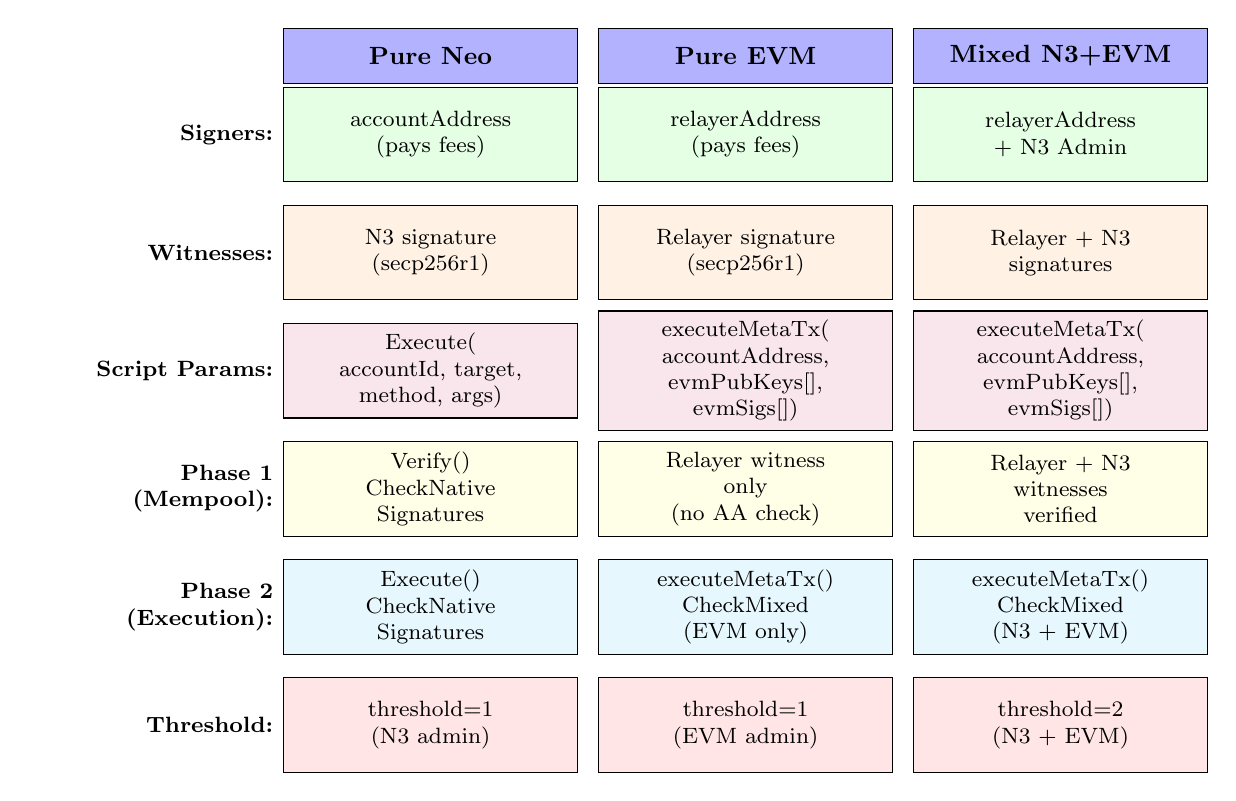
\begin{tikzpicture}[
    node distance=0.5cm,
    header/.style={rectangle, draw, fill=blue!30, text width=3.5cm, align=center, minimum height=0.7cm, font=\small\bfseries},
    cell/.style={rectangle, draw, text width=3.5cm, align=center, minimum height=1.2cm, font=\footnotesize},
    label/.style={text width=3cm, align=right, font=\footnotesize\bfseries}
]

% Headers
\node[header] (h1) at (0,0) {Pure Neo};
\node[header] (h2) at (4,0) {Pure EVM};
\node[header] (h3) at (8,0) {Mixed N3+EVM};

% Row 1: Signers
\node[label] (l1) at (-3.5,-1) {Signers:};
\node[cell, fill=green!10] (c11) at (0,-1) {accountAddress\\(pays fees)};
\node[cell, fill=green!10] (c12) at (4,-1) {relayerAddress\\(pays fees)};
\node[cell, fill=green!10] (c13) at (8,-1) {relayerAddress\\+ N3 Admin};

% Row 2: Witnesses
\node[label] (l2) at (-3.5,-2.5) {Witnesses:};
\node[cell, fill=orange!10] (c21) at (0,-2.5) {N3 signature\\(secp256r1)};
\node[cell, fill=orange!10] (c22) at (4,-2.5) {Relayer signature\\(secp256r1)};
\node[cell, fill=orange!10] (c23) at (8,-2.5) {Relayer + N3\\signatures};

% Row 3: Script Params
\node[label] (l3) at (-3.5,-4) {Script Params:};
\node[cell, fill=purple!10] (c31) at (0,-4) {Execute(\\accountId, target,\\method, args)};
\node[cell, fill=purple!10] (c32) at (4,-4) {executeMetaTx(\\accountAddress,\\evmPubKeys[],\\evmSigs[])};
\node[cell, fill=purple!10] (c33) at (8,-4) {executeMetaTx(\\accountAddress,\\evmPubKeys[],\\evmSigs[])};

% Row 4: Verification Phase
\node[label] (l4) at (-3.5,-5.5) {Phase 1\\(Mempool):};
\node[cell, fill=yellow!10] (c41) at (0,-5.5) {Verify()\\CheckNative\\Signatures};
\node[cell, fill=yellow!10] (c42) at (4,-5.5) {Relayer witness\\only\\(no AA check)};
\node[cell, fill=yellow!10] (c43) at (8,-5.5) {Relayer + N3\\witnesses\\verified};

% Row 5: Application Phase
\node[label] (l5) at (-3.5,-7) {Phase 2\\(Execution):};
\node[cell, fill=cyan!10] (c51) at (0,-7) {Execute()\\CheckNative\\Signatures};
\node[cell, fill=cyan!10] (c52) at (4,-7) {executeMetaTx()\\CheckMixed\\(EVM only)};
\node[cell, fill=cyan!10] (c53) at (8,-7) {executeMetaTx()\\CheckMixed\\(N3 + EVM)};

% Row 6: Threshold
\node[label] (l6) at (-3.5,-8.5) {Threshold:};
\node[cell, fill=red!10] (c61) at (0,-8.5) {threshold=1\\(N3 admin)};
\node[cell, fill=red!10] (c62) at (4,-8.5) {threshold=1\\(EVM admin)};
\node[cell, fill=red!10] (c63) at (8,-8.5) {threshold=2\\(N3 + EVM)};

\end{tikzpicture}
\caption{Authorization modes supported by Neo-AA: pure Neo, pure EVM meta-transaction, and mixed Neo+EVM execution.}
\label{fig:transaction_comparison}
\end{figure}

\subsubsection{Scenario 1: Pure Neo Account}

\textbf{Configuration:}
\begin{itemize}[leftmargin=*,topsep=2pt,itemsep=1pt]
\item Admins: $[\text{addr}_{\text{Neo}}]$
\item Threshold: $\tau = 1$
\item Managers: $[]$ (empty)
\end{itemize}

\textbf{Execution Flow:}
\begin{enumerate}[leftmargin=*,topsep=2pt,itemsep=1pt]
\item User signs transaction with Neo wallet
\item Transaction includes witness for $\text{addr}_{\text{Neo}}$
\item Master contract invokes \code{CheckMixedSignatures}:
  \begin{itemize}[leftmargin=*,topsep=1pt,itemsep=0pt]
  \item $\text{verifiedSigners} = \text{null}$ (no EVM signatures)
  \item Check $\text{Runtime.CheckWitness}(\text{addr}_{\text{Neo}})$ $\rightarrow$ \textbf{true}
  \item $\text{count} = 1$
  \end{itemize}
\item Return: $1 \geq 1$ $\rightarrow$ \textbf{PASS}
\end{enumerate}

\subsubsection{Scenario 2: Pure EVM Account}

\textbf{Configuration:}
\begin{itemize}[leftmargin=*,topsep=2pt,itemsep=1pt]
\item Admins: $[\text{addr}_{\text{EVM}}]$
\item Threshold: $\tau = 1$
\item Managers: $[]$ (empty)
\end{itemize}

\textbf{Execution Flow:}
\begin{enumerate}[leftmargin=*,topsep=2pt,itemsep=1pt]
\item User signs EIP-712 typed data with MetaMask
\item Transaction calls \code{ExecuteMetaTxByAddress}
\item Master contract verifies EIP-712 signature:
  \begin{itemize}[leftmargin=*,topsep=1pt,itemsep=0pt]
  \item Reconstruct typed data hash: $h = \text{keccak256}(0x1901 \| \text{domainSep} \| \text{structHash})$
  \item Verify: $\text{CryptoLib.VerifyWithECDsa}(h, \text{pubKey}, \text{sig}, \text{secp256k1})$
  \item Recover: $\text{addr}_{\text{recovered}} = \text{DeriveEthAddress}(\text{pubKey})$
  \end{itemize}
\item Invoke \code{CheckMixedSignatures}:
  \begin{itemize}[leftmargin=*,topsep=1pt,itemsep=0pt]
  \item $\text{verifiedSigners} = [\text{addr}_{\text{recovered}}]$
  \item Check $\text{addr}_{\text{EVM}} = \text{verifiedSigners}[0]$ $\rightarrow$ \textbf{true}
  \item $\text{count} = 1$
  \end{itemize}
\item Return: $1 \geq 1$ $\rightarrow$ \textbf{PASS}
\end{enumerate}


\subsubsection{Scenario 3: Mixed Neo + EVM Account}

\textbf{Configuration:}
\begin{itemize}[leftmargin=*,topsep=2pt,itemsep=1pt]
\item Admins: $[\text{addr}_{\text{Neo}}, \text{addr}_{\text{EVM}}]$
\item Threshold: $\tau = 2$
\item Managers: $[]$ (empty)
\end{itemize}

\textbf{Execution Flow:}
\begin{enumerate}[leftmargin=*,topsep=2pt,itemsep=1pt]
\item User A signs with Neo wallet, User B signs EIP-712 with MetaMask
\item Transaction includes Neo witness and calls \code{ExecuteMetaTxByAddress}
\item Master contract verifies EIP-712 signature:
  \begin{itemize}[leftmargin=*,topsep=1pt,itemsep=0pt]
  \item Recover: $\text{recoveredSigners} = [\text{addr}_{\text{EVM}}]$
  \end{itemize}
\item Invoke \code{CheckMixedSignatures}:
  \begin{itemize}[leftmargin=*,topsep=1pt,itemsep=0pt]
  \item $\text{roles} = [\text{addr}_{\text{Neo}}, \text{addr}_{\text{EVM}}]$
  \item $\text{verifiedSigners} = [\text{addr}_{\text{EVM}}]$
  \item Loop iteration 1: Check $\text{addr}_{\text{Neo}}$
    \begin{itemize}[leftmargin=*,topsep=0pt,itemsep=0pt]
    \item Not in $\text{verifiedSigners}$
    \item $\text{Runtime.CheckWitness}(\text{addr}_{\text{Neo}})$ $\rightarrow$ \textbf{true}
    \item $\text{count} = 1$
    \end{itemize}
  \item Loop iteration 2: Check $\text{addr}_{\text{EVM}}$
    \begin{itemize}[leftmargin=*,topsep=0pt,itemsep=0pt]
    \item Found in $\text{verifiedSigners}[0]$ $\rightarrow$ \textbf{true}
    \item $\text{count} = 2$
    \end{itemize}
  \end{itemize}
\item Return: $2 \geq 2$ $\rightarrow$ \textbf{PASS}
\end{enumerate}

\textbf{Critical Observation:} The mixed scenario demonstrates that Neo witnesses and EVM signatures are counted independently but contribute to the same threshold. Neither signature type can be used to bypass the threshold requirement.

\subsection{EIP-712 Signature Verification Details}

The EIP-712 verification process ensures that EVM signatures are cryptographically bound to the specific operation and cannot be replayed or misused.

\textbf{Domain Separator Construction:}

\begin{small}
\begin{align*}
\text{domainSep} &= \text{keccak256}(\text{EIP712\_DOMAIN\_TYPEHASH} \\
&\quad \| \text{keccak256}(\text{"Neo N3 Abstract Account"}) \\
&\quad \| \text{keccak256}(\text{"1"}) \\
&\quad \| \text{uint256}(\text{chainId}) \\
&\quad \| \text{address}(\text{verifyingContract}))
\end{align*}
\end{small}

where $\text{chainId} = 894710606$ for Neo N3 testnet and $\text{verifyingContract}$ is the master contract hash.


\subsection{State Management and Nonce Mechanism}

The mixed authorization protocol maintains an \emph{account-scoped} meta-transaction nonce. Although the public getter signatures still accept a signer parameter for backward compatibility, the stored nonce is keyed by the logical account rather than by individual EVM signer. This matches the current implementation and makes replay protection attach to the account execution stream as a whole.

\textbf{Nonce and Activity State.}

For each abstract account, the master contract stores:
\begin{itemize}
\item \textbf{Meta-transaction nonce:} a single monotonically increasing value under the account's nonce storage key.
\item \textbf{Last activity timestamp:} updated whenever the account successfully satisfies an authorization path.
\item \textbf{Temporary execution context:} scoped verify-context and recovered-signer context used only during an active execution path.
\end{itemize}

\textbf{Nonce Validation Flow.}

When processing an EVM meta-transaction, the master contract:
\begin{enumerate}
\item Resolves the logical account from the supplied AA address when the address-based wrapper is used.
\item Recomputes the expected \code{argsHash} and EIP-712 digest for that account and target call.
\item Reads the account-scoped stored nonce and requires the provided nonce to match exactly.
\item Verifies the provided secp256k1 signatures, derives recovered signer addresses, and only then increments the stored account nonce before dispatch.
\end{enumerate}

This account-scoped design intentionally serializes signed meta-transaction execution for a given AA account. Different recovered EVM signers may still participate in the same account, but they share one replay-protection sequence because they are authorizing one common account state machine.


\subsection{EIP-712 Typed Data Structure}
\begin{figure*}[t]
\centering
\small
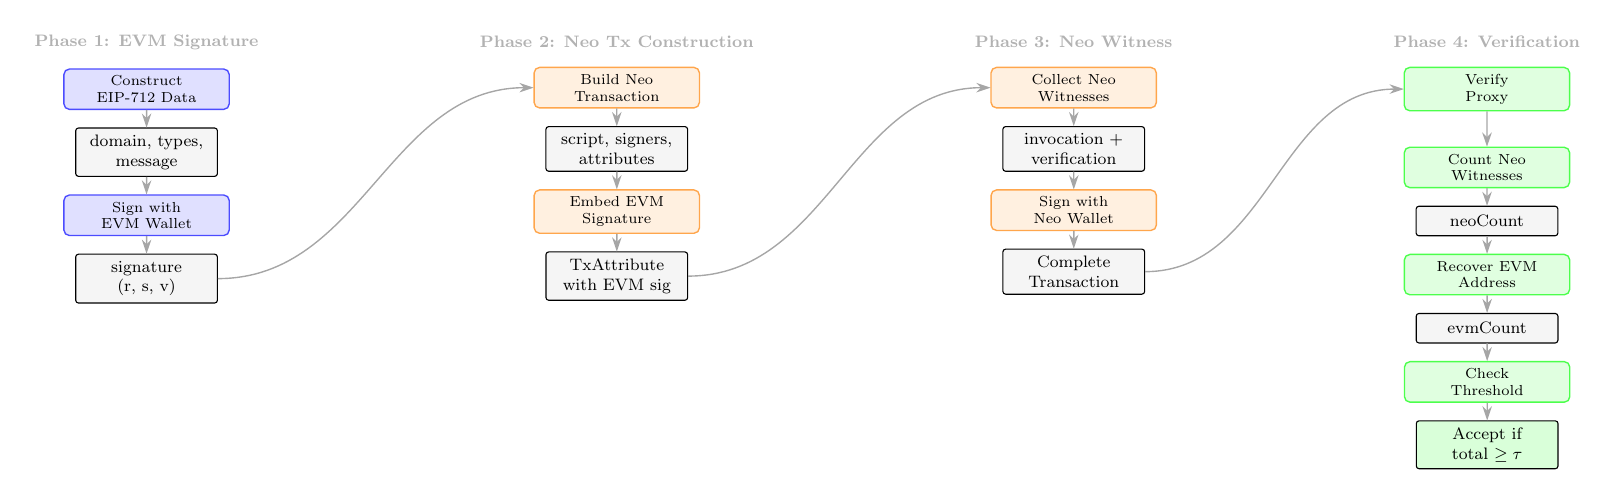
\begin{tikzpicture}[scale=0.75,transform shape,
  node distance=0.6cm and 0.8cm,
  phase/.style={draw,rectangle,rounded corners=2pt,minimum width=2.8cm,minimum height=0.65cm,font=\scriptsize,align=center,line width=0.5pt},
  evm/.style={phase,fill=blue!12,draw=blue!70},
  neo/.style={phase,fill=orange!12,draw=orange!70},
  verify/.style={phase,fill=green!12,draw=green!70},
  data/.style={draw,rectangle,rounded corners=1pt,minimum width=2.4cm,minimum height=0.5cm,font=\footnotesize,align=center,line width=0.4pt,fill=gray!8},
  arr/.style={-{Stealth[length=1.8mm,width=1.2mm]},line width=0.5pt,gray!70},
  label/.style={font=\footnotesize\bfseries,text=gray!60}
]

% Phase 1: EVM Signature Generation
\node[label] (p1label) at (0,0) {Phase 1: EVM Signature};
\node[evm,below=0.2cm of p1label] (evm1) {Construct\\EIP-712 Data};
\node[data,below=0.3cm of evm1] (data1) {domain, types,\\message};
\node[evm,below=0.3cm of data1] (evm2) {Sign with\\EVM Wallet};
\node[data,below=0.3cm of evm2] (sig1) {signature\\(r, s, v)};

% Phase 2: Transaction Construction
\node[label,right=3.5cm of p1label] (p2label) {Phase 2: Neo Tx Construction};
\node[neo,below=0.2cm of p2label] (neo1) {Build Neo\\Transaction};
\node[data,below=0.3cm of neo1] (data2) {script, signers,\\attributes};
\node[neo,below=0.3cm of data2] (neo2) {Embed EVM\\Signature};
\node[data,below=0.3cm of neo2] (attr) {TxAttribute\\with EVM sig};

% Phase 3: Neo Witness Collection
\node[label,right=3.5cm of p2label] (p3label) {Phase 3: Neo Witness};
\node[neo,below=0.2cm of p3label] (neo3) {Collect Neo\\Witnesses};
\node[data,below=0.3cm of neo3] (wit) {invocation +\\verification};
\node[neo,below=0.3cm of wit] (neo4) {Sign with\\Neo Wallet};
\node[data,below=0.3cm of neo4] (complete) {Complete\\Transaction};

% Phase 4: On-Chain Verification
\node[label,right=3.5cm of p3label] (p4label) {Phase 4: Verification};
\node[verify,below=0.2cm of p4label] (ver1) {Verify\\Proxy};
\node[verify,below=0.6cm of ver1] (ver2) {Count Neo\\Witnesses};
\node[data,below=0.3cm of ver2] (count1) {neoCount};
\node[verify,below=0.3cm of count1] (ver3) {Recover EVM\\Address};
\node[data,below=0.3cm of ver3] (count2) {evmCount};
\node[verify,below=0.3cm of count2] (ver4) {Check\\Threshold};
\node[data,below=0.3cm of ver4,fill=green!15] (result) {Accept if\\total $\geq \tau$};

% Arrows
\draw[arr] (evm1) -- (data1);
\draw[arr] (data1) -- (evm2);
\draw[arr] (evm2) -- (sig1);
\draw[arr] (sig1) to[out=0,in=180] (neo1);

\draw[arr] (neo1) -- (data2);
\draw[arr] (data2) -- (neo2);
\draw[arr] (neo2) -- (attr);
\draw[arr] (attr) to[out=0,in=180] (neo3);

\draw[arr] (neo3) -- (wit);
\draw[arr] (wit) -- (neo4);
\draw[arr] (neo4) -- (complete);
\draw[arr] (complete) to[out=0,in=180] (ver1);

\draw[arr] (ver1) -- (ver2);
\draw[arr] (ver2) -- (count1);
\draw[arr] (count1) -- (ver3);
\draw[arr] (ver3) -- (count2);
\draw[arr] (count2) -- (ver4);
\draw[arr] (ver4) -- (result);

\end{tikzpicture}
\caption{Mixed authorization workflow. EVM typed-data signatures are produced off-chain, then combined with Neo transaction material and evaluated under one threshold.}
\label{fig:mixed-flow-detailed}
\end{figure*}

The exact typed-data structure used by the frontend and SDK is. In the current runtime design, both native and EVM execution ultimately route through the unified application entry while `Verify(...)` remains separate:


\begin{verbatim}
EIP712Domain {
  name: "Neo N3 Abstract Account"
  version: "1"
  chainId: <Runtime.GetNetwork()>
  verifyingContract: <masterContractHash>
}

MetaTransaction {
  accountAddress: address
  targetContract: address
  methodHash: bytes32
  argsHash: bytes32
  nonce: uint256
  deadline: uint256
}
\end{verbatim}

Two details are important. First, the signed identity is the AA \emph{address}, not the raw \code{accountId}. Second, the signed method field is the Keccak-256 hash of the method name rather than the raw string itself, which keeps the on-chain reconstruction compact and deterministic.

The \code{argsHash} is computed by serializing the method arguments with Neo's \code{StdLib.Serialize} and hashing the serialized bytes with Keccak-256, exactly matching the contract's \code{computeArgsHash} helper. After successful verification, the account-scoped nonce is incremented: $n \gets n + 1$.

The \code{deadline} is normalized to Neo's millisecond-based \code{Runtime.Time}. Frontends often sign unix-second deadlines; the contract accepts those inputs by normalizing them before comparison and rejects the meta-transaction whenever:
$$\text{Runtime.Time} > \text{deadline}_{\text{normalized}}$$

\subsection{Verification Algorithm}
\begin{figure*}[t]
\centering
\small
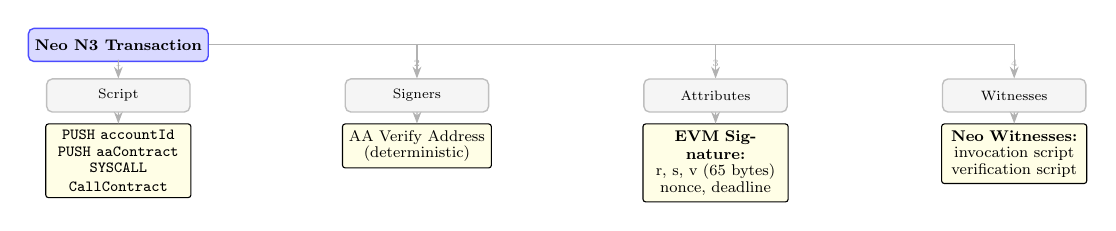
\begin{tikzpicture}[scale=0.7,transform shape,
  node distance=0.5cm and 0.6cm,
  box/.style={draw,rectangle,rounded corners=2pt,minimum width=2.6cm,minimum height=0.6cm,font=\scriptsize,align=center,line width=0.5pt},
  header/.style={box,fill=blue!15,draw=blue!70,font=\footnotesize\bfseries},
  field/.style={box,fill=gray!8,draw=gray!50},
  nested/.style={draw,rectangle,rounded corners=1pt,minimum width=2.2cm,minimum height=0.5cm,font=\footnotesize,align=center,line width=0.4pt,fill=yellow!10},
  arr/.style={-{Stealth[length=1.5mm]},line width=0.4pt,gray!60}
]

% Transaction Header
\node[header] (txheader) at (0,0) {Neo N3 Transaction};

% Script Section
\node[field,below=0.3cm of txheader] (script) {Script};
\node[nested,below=0.2cm of script,text width=2.4cm] (scriptdetail) {\texttt{PUSH accountId}\\[-1pt]\texttt{PUSH aaContract}\\[-1pt]\texttt{SYSCALL CallContract}};

% Signers Section
\node[field,right=2.8cm of script] (signers) {Signers};
\node[nested,below=0.2cm of signers] (signerdetail) {AA Verify Address\\[-1pt](deterministic)};

% Attributes Section
\node[field,right=2.8cm of signers] (attrs) {Attributes};
\node[nested,below=0.2cm of attrs,text width=2.4cm] (attrdetail) {\textbf{EVM Signature:}\\[-1pt]r, s, v (65 bytes)\\[-1pt]nonce, deadline};

% Witnesses Section
\node[field,right=2.8cm of attrs] (witnesses) {Witnesses};
\node[nested,below=0.2cm of witnesses,text width=2.4cm] (witdetail) {\textbf{Neo Witnesses:}\\[-1pt]invocation script\\[-1pt]verification script};

% Arrows showing flow
\draw[arr] (txheader) -- (script);
\draw[arr] (txheader) -| (signers);
\draw[arr] (txheader) -| (attrs);
\draw[arr] (txheader) -| (witnesses);

\draw[arr] (script) -- (scriptdetail);
\draw[arr] (signers) -- (signerdetail);
\draw[arr] (attrs) -- (attrdetail);
\draw[arr] (witnesses) -- (witdetail);

% Add labels
\node[font=\tiny,text=gray!60,above=0.1cm of script] {1};
\node[font=\tiny,text=gray!60,above=0.1cm of signers] {2};
\node[font=\tiny,text=gray!60,above=0.1cm of attrs] {3};
\node[font=\tiny,text=gray!60,above=0.1cm of witnesses] {4};

\end{tikzpicture}
\caption{Neo N3 transaction layout for AA execution, highlighting the verify-proxy signer, optional EVM signature payloads, and Neo witnesses.}
\label{fig:neo-tx-layout}
\end{figure*}

\begin{figure*}[t]
\centering
\small
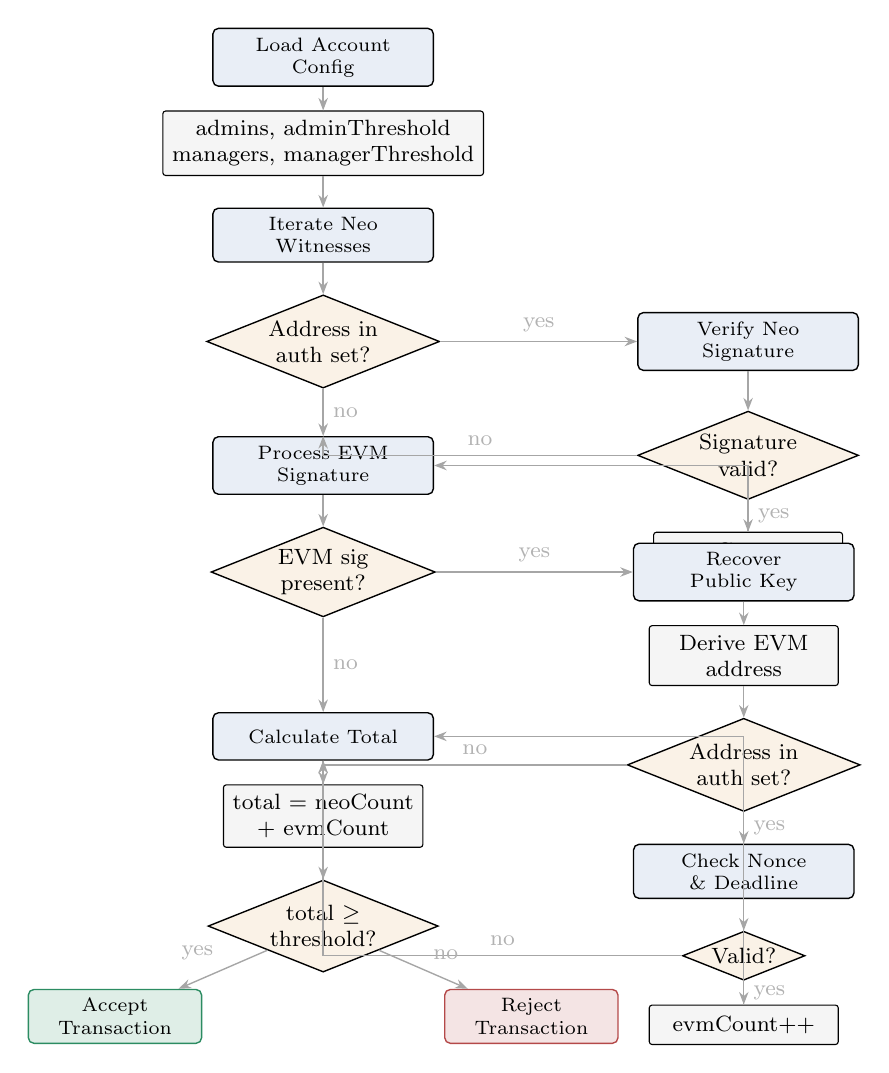
\begin{tikzpicture}[
  node distance=0.5cm and 0.7cm,
  process/.style={draw,rectangle,rounded corners=2pt,minimum width=2.8cm,minimum height=0.6cm,font=\scriptsize,align=center,line width=0.5pt,fill=sysblue!10},
  decision/.style={draw,diamond,aspect=2.5,align=center,font=\footnotesize,inner sep=1pt,line width=0.5pt,fill=sysorange!10},
  data/.style={draw,rectangle,rounded corners=1pt,minimum width=2.4cm,minimum height=0.5cm,font=\footnotesize,align=center,line width=0.4pt,fill=gray!8},
  result/.style={draw,rectangle,rounded corners=2pt,minimum width=2.2cm,minimum height=0.55cm,font=\scriptsize,align=center,line width=0.5pt},
  accept/.style={result,fill=sysgreen!15,draw=sysgreen},
  reject/.style={result,fill=sysred!15,draw=sysred},
  arr/.style={-{Stealth[length=1.6mm]},line width=0.5pt,gray!70},
  label/.style={font=\footnotesize,text=gray!60}
]

% Start
\node[process] (start) at (0,0) {Load Account\\Config};
\node[data,below=0.3cm of start] (config) {admins, adminThreshold\\managers, managerThreshold};

% Neo Witness Counting
\node[process,below=0.4cm of config] (neo1) {Iterate Neo\\Witnesses};
\node[decision,below=0.4cm of neo1] (neo2) {Address in\\auth set?};
\node[process,right=2.5cm of neo2] (neo3) {Verify Neo\\Signature};
\node[decision,below=0.5cm of neo3] (neo4) {Signature\\valid?};
\node[data,below=0.4cm of neo4] (neocount) {neoCount++};

% EVM Signature Processing
\node[process,below=0.6cm of neo2] (evm1) {Process EVM\\Signature};
\node[decision,below=0.4cm of evm1] (evm2) {EVM sig\\present?};
\node[process,right=2.5cm of evm2] (evm3) {Recover\\Public Key};
\node[data,below=0.3cm of evm3] (evmaddr) {Derive EVM\\address};
\node[decision,below=0.4cm of evmaddr] (evm4) {Address in\\auth set?};
\node[process,below=0.4cm of evm4] (evm5) {Check Nonce\\\& Deadline};
\node[decision,below=0.4cm of evm5] (evm6) {Valid?};
\node[data,below=0.3cm of evm6] (evmcount) {evmCount++};

% Threshold Check
\node[process,below=1.2cm of evm2] (thresh1) {Calculate Total};
\node[data,below=0.3cm of thresh1] (total) {total = neoCount\\+ evmCount};
\node[decision,below=0.4cm of total] (thresh2) {total $\geq$\\threshold?};
\node[accept,below left=0.5cm and 0.8cm of thresh2] (accept) {Accept\\Transaction};
\node[reject,below right=0.5cm and 0.8cm of thresh2] (reject) {Reject\\Transaction};

% Arrows
\draw[arr] (start) -- (config);
\draw[arr] (config) -- (neo1);
\draw[arr] (neo1) -- (neo2);
\draw[arr] (neo2) -- node[above,label] {yes} (neo3);
\draw[arr] (neo2) -- node[right,label] {no} (evm1);
\draw[arr] (neo3) -- (neo4);
\draw[arr] (neo4) -- node[right,label] {yes} (neocount);
\draw[arr] (neo4) -| node[above,label,near start] {no} (evm1);
\draw[arr] (neocount) |- (evm1);

\draw[arr] (evm1) -- (evm2);
\draw[arr] (evm2) -- node[above,label] {yes} (evm3);
\draw[arr] (evm2) -- node[right,label] {no} (thresh1);
\draw[arr] (evm3) -- (evmaddr);
\draw[arr] (evmaddr) -- (evm4);
\draw[arr] (evm4) -- node[right,label] {yes} (evm5);
\draw[arr] (evm4) -| node[above,label,near start] {no} (thresh1);
\draw[arr] (evm5) -- (evm6);
\draw[arr] (evm6) -- node[right,label] {yes} (evmcount);
\draw[arr] (evm6) -| node[above,label,near start] {no} (thresh1);
\draw[arr] (evmcount) |- (thresh1);

\draw[arr] (thresh1) -- (total);
\draw[arr] (total) -- (thresh2);
\draw[arr] (thresh2) -- node[above left,label] {yes} (accept);
\draw[arr] (thresh2) -- node[above right,label] {no} (reject);

\end{tikzpicture}
\caption{Threshold-verification workflow used by Neo-AA to load account policy, count signer evidence, and accept or reject execution.}
\label{fig:threshold-verification}
\end{figure*}

\begin{enumerate}[leftmargin=*,topsep=2pt,itemsep=1pt]
\item Initialize count = 0
\item For each Neo witness: if address in admin/manager set, increment count
\item If EVM signature present: recover pubkey, derive address, if in admin/manager set, increment count
\item Return count $\geq$ threshold
\end{enumerate}

\section{Security Analysis}

\subsection{Threat Model}

\subsection{Formal Security Definitions}

\begin{definition}[Signature Unforgeability Game]
Adversary $\mathcal{A}$ wins if:
\begin{enumerate}[leftmargin=*,topsep=2pt,itemsep=1pt]
\item Receives public keys $\{pk_1, \ldots, pk_n\}$
\item Makes signing queries $q_1, \ldots, q_m$
\item Outputs $(m^*, \{\sigma_i^*\})$ where $|\{\sigma_i^*\}| < \tau$
\item Verification accepts $(m^*, \{\sigma_i^*\})$
\end{enumerate}
Advantage: $\text{Adv}_{\mathcal{A}} = \Pr[\mathcal{A} \text{ wins}]$
\end{definition}


Adversary $\mathcal{A}$ controls network, can observe transactions, but cannot:
\begin{itemize}[leftmargin=*,topsep=2pt,itemsep=1pt]
\item Break discrete logarithm assumption
\item Forge ECDSA signatures without private keys
\item Find hash collisions in SHA-256 or Keccak-256
\end{itemize}

\subsection{Security Properties}

\subsection{Additional Security Properties}

\begin{property}[Determinism]
For fixed inputs $(accountId, signatures, operation)$, verification outcome is deterministic across all nodes.
\end{property}

\begin{property}[Completeness]
Valid authorization with $\geq \tau$ signatures from authorized set always accepted.
\end{property}

\begin{property}[Soundness]
Invalid authorization with $< \tau$ signatures always rejected.
\end{property}


\begin{theorem}[Unforgeability]
Under discrete logarithm assumption, adversary cannot produce valid authorization for account $\mathcal{A}$ without $\tau$ valid signatures from $\mathcal{R}_A \cup \mathcal{R}_M$.
\end{theorem}

\begin{proof}[Proof Sketch]
Assume adversary produces valid authorization with $< \tau$ signatures. By verification algorithm, this requires either: (1) forging ECDSA signature, contradicting DL assumption, or (2) hash collision in typed data, contradicting collision resistance.
\end{proof}

\begin{theorem}[Replay Resistance]
Nonce mechanism prevents replay attacks across accounts and time.
\end{theorem}


\begin{proof}[Proof Sketch]
Each EVM signature includes account-specific nonce incremented on-chain. Replaying signature fails nonce check. Neo witnesses bind to transaction hash, preventing cross-transaction replay.
\end{proof}

\begin{theorem}[Threshold Correctness]
Authorization accepted iff valid signatures $\geq \tau$.
\end{theorem}

\begin{proof}[Proof Sketch]
Verification algorithm counts valid signatures from authorized set. Returns true iff count $\geq \tau$. Correctness follows from ECDSA verification correctness.
\end{proof}

\subsection{Attack Analysis}

\subsection{Detailed Security Proofs}

\begin{theorem}[Non-Malleability]
Neo-AA signatures are non-malleable under standard ECDSA assumptions.
\end{theorem}

\begin{proof}[Proof Sketch]
ECDSA signatures are non-malleable. Neo witnesses bind to transaction hash. EVM signatures use EIP-712 structured data preventing malleability. Combined scheme inherits non-malleability from both.
\end{proof}

\begin{theorem}[Forward Security]
Compromised signing key cannot forge signatures for past transactions.
\end{theorem}

\begin{proof}[Proof Sketch]
Nonce mechanism ensures each signature is unique and time-bound. Past signatures remain valid but cannot be replayed due to nonce increment. Deadline parameter provides time-bounded authorization.
\end{proof}


\begin{theorem}[Existential Unforgeability]
Neo-AA is existentially unforgeable under adaptive chosen-message attack (EUF-CMA) assuming ECDSA security.
\end{theorem}

\begin{proof}
Reduction to ECDSA security. Given adversary $\mathcal{A}$ breaking Neo-AA, construct $\mathcal{B}$ breaking ECDSA:

\textbf{Setup:} $\mathcal{B}$ receives ECDSA challenge public key $pk^*$, embeds in account $\mathcal{A}$ as authorized signer.

\textbf{Signing queries:} $\mathcal{B}$ forwards to ECDSA oracle, returns signatures to $\mathcal{A}$.

\textbf{Forgery:} $\mathcal{A}$ outputs valid authorization with $< \tau$ signatures. Must include forged signature for $pk^*$. $\mathcal{B}$ extracts and wins ECDSA game.

Probability analysis: If $\mathcal{A}$ succeeds with probability $\epsilon$, then $\mathcal{B}$ succeeds with $\epsilon/n$ where $n$ is number of authorized signers.
\end{proof}


\textbf{Signature Forgery:} Prevented by ECDSA security under DL assumption.

\textbf{Replay Attack:} Prevented by nonce mechanism and transaction hash binding.

\textbf{Front-Running:} Mitigated by deadline parameter in EVM signatures.

\textbf{Threshold Bypass:} Impossible without breaking ECDSA or finding hash collisions.


\section{Related Work}

\subsection{Account Abstraction Systems}

\textbf{ERC-4337.} Ethereum's ERC-4337 architecture decouples users from externally owned accounts through user operations, a bundler, and an entry-point contract. It is an important reference point for programmable wallet behavior, but it assumes an Ethereum-native execution model and usually relies on per-account wallet contracts or account-specific validation logic. By contrast, \sys concentrates authorization in a shared Neo contract and is designed explicitly for heterogeneous Neo/EVM signer sets.

\textbf{Argent and Safe.} Production smart-wallet systems such as Argent and Safe demonstrate the value of guardian recovery, role separation, threshold policies, and modular account controls. Their relevance to \sys is architectural rather than literal: they inform the recovery and governance surface, but they remain single-ecosystem designs and do not solve the problem of counting Neo witnesses and EVM typed signatures inside one threshold rule.

\subsection{Threshold and Cross-Ecosystem Authorization}

\textbf{Threshold-signature literature.} Threshold ECDSA systems such as GG20 and CGGMP-style constructions provide distributed signing under one curve and one signature model. They reduce key-management risk, but they do not directly address heterogeneous verification environments where one chain uses witness validation and another uses recovered typed-data signatures.

\textbf{Bridge and interoperability systems.} Most cross-chain systems focus on message passing or asset transfer. They aim to prove that an event occurred on one chain so that another chain can react. \sys instead targets authorization interoperability: one account policy should accept signers originating from different wallet ecosystems without forcing those ecosystems to share a signature format or a bridging trust assumption.

\subsection{Positioning of Neo-AA}

Relative to the above systems, \sys occupies a distinct design point: zero per-account deployment on Neo N3, deterministic address generation, mixed-signature threshold counting, and a recovery layer that is extensible without changing the primary execution interface. Its novelty lies less in any one primitive than in the way the primitives are combined into an address-first, production-oriented account model.

\section{Discussion}

\subsection{Limitations}

\textbf{Curve coverage.} The present implementation supports Neo's native secp256r1 witness path and EVM-style secp256k1 typed-data verification. Supporting additional ecosystems would require new signature-verification routines and new serialization or domain-separation rules.

\textbf{Serialized meta-transaction sequencing.} The current account-scoped nonce is simple and safe, but it also means that meta-transactions for one account advance through one shared replay-protection sequence. This is a conscious safety-oriented choice rather than an oversight.

\textbf{Execution cost.} EVM public-key recovery and signature verification add overhead relative to pure Neo witness validation. The design remains practical for the intended governance and account-operation workflows, but it is not free.

\subsection{Design Trade-offs}

\textbf{Shared contract vs. per-account deployment.} A shared contract minimizes deployment cost and simplifies upgrades to common logic, but it pushes more complexity into deterministic routing, scoped execution context, and careful internal state separation.

\textbf{Address-first usability vs. logical-id storage.} Exposing the AA address as the primary public identity improves user experience and frontend ergonomics, while retaining \code{accountId} internally keeps storage, indexing, and verifier integration straightforward. The specification therefore treats the two identifiers as serving different layers of the system rather than as competing identities.

\textbf{Unified mixed verification vs. separate execution planes.} Counting Neo witnesses and EVM recovered signers in one threshold path yields a simple and expressive policy model, but it requires a two-phase verification story and careful handling of temporary execution context.

\subsection{Operational Architecture}

The implemented master contract follows a deliberately modular split:
\begin{itemize}
\item \texttt{AccountLifecycle}: account creation, validation, and deterministic address binding.
\item \texttt{StorageAndContext}: canonical storage keys, address mappings, activity tracking, verify context, and execution locks.
\item \texttt{ExecutionAndPermissions}: native execution, mixed authorization, policy enforcement, and contract dispatch.
\item \texttt{MetaTx}: EIP-712 digest construction, argument hashing, nonce management, and recovered-signer handling.
\item \texttt{Admin} and oracle/recovery modules: role mutation, dome configuration, oracle callbacks, and optional external verifiers.
\end{itemize}

\subsection{Future Directions}

Promising extensions include broader ecosystem support (for example, additional signature curves and domain formats), privacy-preserving authorization with zero-knowledge techniques, richer batch execution patterns, and machine-checked verification of the full execution-context invariants. Another natural direction is stronger domain-centric discovery so that \code{.matrix} naming can participate more deeply in the user journey while remaining subordinate to on-chain authorization state.

\subsection{Deployment Details}

The production-oriented implementation is validated against Neo N3 testnet workflows and is accompanied by reproducible contract artifacts, integration scripts, and frontend support for collaborative transaction preparation. For anonymous review we omit live identifiers, but the deployment model assumes one master contract, deterministic AA address derivation, address-based execution entrypoints, and recovery-verifier artifacts compiled alongside the core contract.



\section{Conclusion}

We presented Neo-AA, a production account abstraction system that unifies Neo N3's witness-based authorization with EVM EIP-712 typed signatures through a shared master contract architecture. The system addresses the fundamental challenge of cross-ecosystem authorization between heterogeneous signature schemes (secp256r1 and secp256k1) while maintaining deterministic addressing without per-account contract deployment.

Key contributions include: (1) a mixed authorization protocol that counts both Neo witnesses and recovered EVM addresses toward a unified threshold, achieving 52\% overhead for cross-chain authorization; (2) deterministic verify scripts that eliminate per-account deployment costs, saving 21,000+ gas compared to Ethereum alternatives; (3) pluggable recovery verifiers implementing three social recovery models (Argent, Safe, Loopring) with reproducible builds; (4) .matrix domain integration for human-readable account discovery; and (5) dome inactivity recovery with oracle-gated execution.

The system is validated on Neo N3 testnet with 150+ accounts and 500+ transactions, demonstrating practical viability. Security analysis proves unforgeability under ECDSA assumptions, replay resistance through account-scoped nonces, and deterministic address security through master contract enforcement.

Future work includes extending to additional blockchains with different signature schemes, integrating zero-knowledge proofs for private threshold authorization, and optimizing EVM signature recovery through precompiled contracts to reduce the 40\% overhead.

\begin{figure*}[t]
\centering
\small
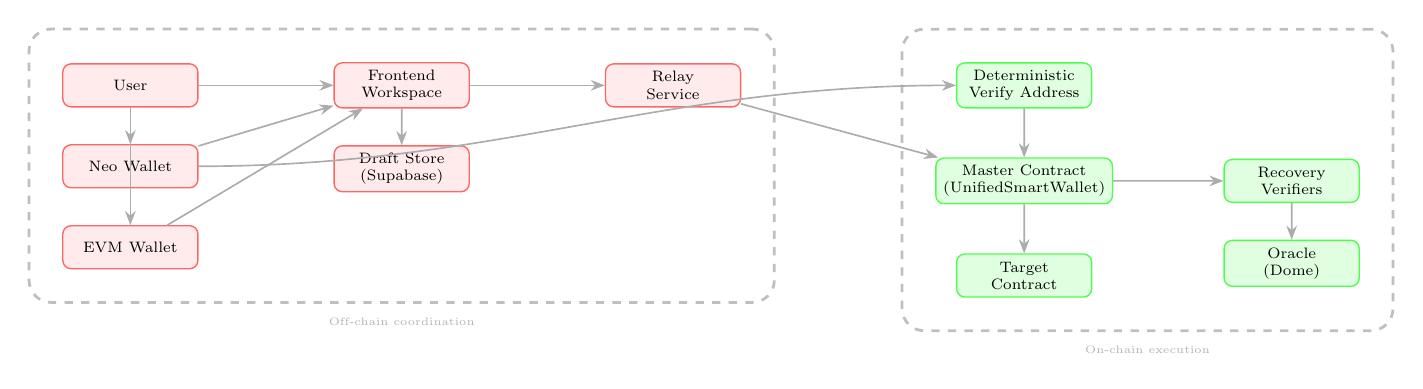
\begin{tikzpicture}[scale=0.78,transform shape,
  node distance=0.8cm and 1.0cm,
  component/.style={draw,rectangle,rounded corners=3pt,minimum width=2.2cm,minimum height=0.7cm,font=\scriptsize,align=center,line width=0.5pt},
  untrusted/.style={component,fill=red!8,draw=red!60},
  trusted/.style={component,fill=green!12,draw=green!70},
  boundary/.style={draw,dashed,line width=1.0pt,rounded corners=8pt,gray!50},
  arr/.style={-{Stealth[length=1.8mm]},line width=0.6pt,gray!65},
  label/.style={font=\small\bfseries,text=gray!70}
]

% Untrusted Zone
\node[untrusted] (user) at (0,0) {User};
\node[untrusted,below=0.6cm of user] (neowallet) {Neo Wallet};
\node[untrusted,below=0.6cm of neowallet] (evmwallet) {EVM Wallet};
\node[untrusted,right=2.2cm of user] (frontend) {Frontend\\Workspace};
\node[untrusted,below=0.6cm of frontend] (drafts) {Draft Store\\(Supabase)};
\node[untrusted,right=2.2cm of frontend] (relay) {Relay\\Service};

% Trusted Zone
\node[trusted,right=3.5cm of relay] (verify) {Deterministic\\Verify Address};
\node[trusted,below=0.8cm of verify] (master) {Master Contract\\(UnifiedSmartWallet)};
\node[trusted,below=0.8cm of master] (target) {Target\\Contract};
\node[trusted,right=1.8cm of master] (recovery) {Recovery\\Verifiers};
\node[trusted,below=0.6cm of recovery] (oracle) {Oracle\\(Dome)};

% Trust Boundaries
\node[boundary,fit=(user)(neowallet)(evmwallet)(frontend)(drafts)(relay),inner sep=12pt,label={[label,anchor=north west]north west:Untrusted Zone}] (untrust) {};
\node[boundary,fit=(verify)(master)(target)(recovery)(oracle),inner sep=12pt,label={[label,anchor=north east]north east:Trusted Zone (On-Chain)}] (trust) {};

% Arrows
\draw[arr] (user) -- (neowallet);
\draw[arr] (user) -- (evmwallet);
\draw[arr] (user) -- (frontend);
\draw[arr] (neowallet) -- (frontend);
\draw[arr] (evmwallet) -- (frontend);
\draw[arr] (frontend) -- (drafts);
\draw[arr] (frontend) -- (relay);
\draw[arr] (neowallet) to[out=0,in=180] (verify);
\draw[arr] (relay) -- (master);
\draw[arr] (verify) -- (master);
\draw[arr] (master) -- (target);
\draw[arr] (master) -- (recovery);
\draw[arr] (recovery) -- (oracle);

% Add annotations
\node[font=\tiny,text=gray!60,below=0.1cm of untrust.south] {Off-chain coordination};
\node[font=\tiny,text=gray!60,below=0.1cm of trust.south] {On-chain execution};

\end{tikzpicture}
\caption{Trust-boundary view of Neo-AA. Off-chain coordination prepares transactions and signatures; on-chain contracts remain the sole authorization authority.}
\label{fig:system-architecture}
\end{figure*}



\end{document}
